\chapter{绪论}
\label{chp1}

\section{雷达的基本概念}
\textbf{雷达}(Radar)是英文 Radio Detection and Ranging的缩写的英译,即用无线电波的反射信号发现目标并测定其空间位置、移动方向、速度、相对距离甚至大概形状的电子设备。作为一种重要的探测手段,雷达被广泛应用于航空与航海导航、军事侦察和预警、气象观测以及太空探索等领域。

严格来说,雷达的研发工作始于20世纪30年代,最初是为探测敌方飞机和舰船而设计的,而其基本概念则可追溯到19世纪末期电磁波反射实验的发现。在1864年,麦克斯韦(James Clerk Maxwell)提出了电磁波的理论,给出了著名的麦克斯韦方程组,从理论上证明了光是一种特殊的电磁波。该理论的一个延伸是,电磁波也可以像光一样被金属物体反射、被电介质折射。随后赫兹(Heinrich Hertz)在1887年使用波长为66厘米(对应于大约 455MHz)的无线电波成功地实验验证了这一结论,并于1888年发表了相关论文。

实验装置如\cref{fig_chp1_hertz}所示,主要由一个发射天线和一个接收天线组成。其中发射天线是由两个带有金属杆的黄铜球构成,金属杆之间留有一个小间隙。当接通电源时,电流在金属棒之间产生振荡,从而在空间中产生无线电波。这些无线电波会在空间中传播,并被金属板反射回来,形成驻波。接收天线则是一个有开口的金属环,它可以接收到反射回来的无线电波,并在开口处产生火花。通过移动接收天线的位置,可以观察到火花的强度变化,从而得到无线电波的波长,结合频率可以计算出电磁波的传播速度,进而验证麦克斯韦方程组的正确性。

\begin{figure}[htb!]
    \centering
    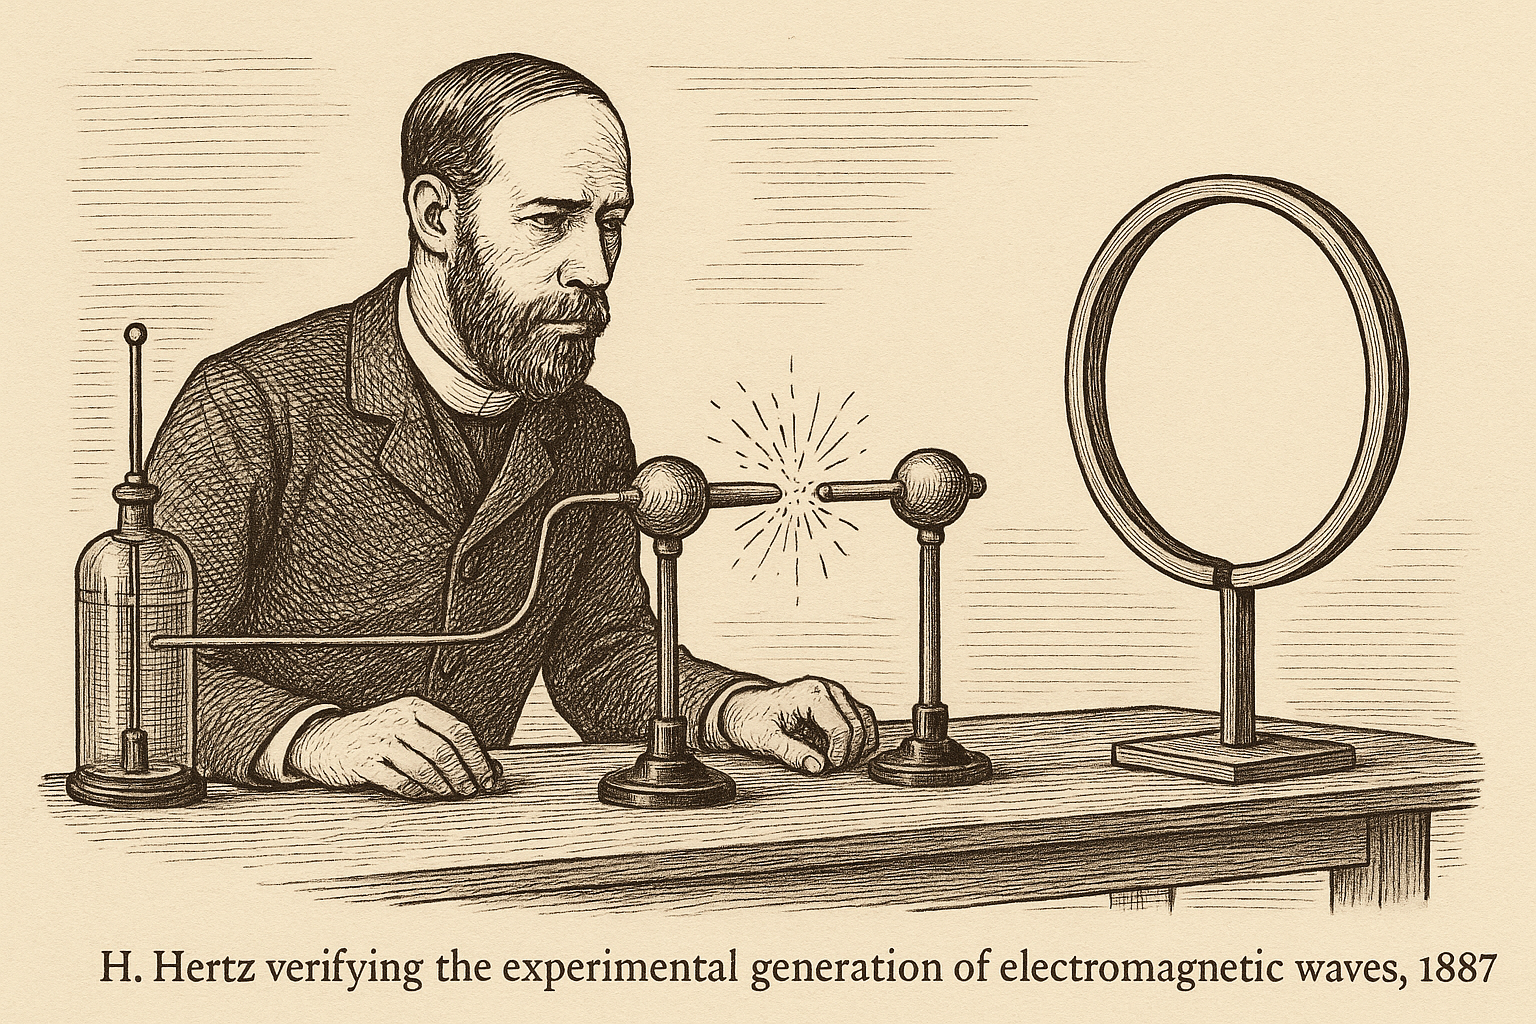
\includegraphics[width=.6\textwidth]{./img/intro/hertz_experiment.png}
    \caption{赫兹的实验装置示意图}
    \label{fig_chp1_hertz}
\end{figure}

雷达利用的便是电磁波的反射特性,通过发射电磁波并接收其反射信号来探测目标物体的位置、方向和速度等信息。雷达系统通常包括发射机、天线、接收机和信号处理单元等部分。发射机产生高频电磁波信号,通过天线向外发射。当电磁波遇到目标物体时,会发生反射,反射信号被天线接收并传输到接收机进行处理。通过分析反射信号的时间延迟和频率变化等特征,可以计算出目标物体的距离、速度和方向等信息。

\section{雷达工作原理}

\subsection{基本组成}
雷达系统的主要组成部分包括发射机、接收机、天线、波形产生器和信号处理单元,如\cref{fig_chp1_radar_system}所示。

\begin{figure}[htb!]
    \centering
    % \includegraphics[width=.4\textwidth]{./img}
    \begin{tikzpicture}
        \tikzset{
            myblock/.style={
                    rectangle, draw, minimum width=2cm, minimum height=1cm, rounded corners, thick
                }
        }

        \node (transmitter) [myblock, fill=c1!60] at (0, 0) {发射机};
        \node (receiver) [myblock, fill=c2!60] at (0, -3) {接收机};
        \node (antenna) [myblock, fill=c3!60] at (-3, -1.5) {天线};
        \node (waveform_generator) [myblock, fill=c4!60] at (3, 0) {波形产生器};
        \node (signal_processing) [myblock, fill=c5!60] at (3, -3) {信号处理单元};

        \draw[-latex, thick] (transmitter) -- (antenna);
        \draw[-latex, thick] (antenna) -- (receiver);
        \draw[-latex, thick] (receiver) -- (signal_processing);
        \draw[-latex, thick] (waveform_generator) -- (transmitter);
    \end{tikzpicture}
    \caption{雷达系统的基本组成}
    \label{fig_chp1_radar_system}
\end{figure}

整个雷达系统的工作流程如下:
\begin{enumerate}
    \item \textbf{波形产生}:波形产生器生成特定的电磁波信号,通常是脉冲信号或连续波信号。
    \item \textbf{发射}:发射机将生成的电磁波信号放大,并通过天线向外发射。
    \item \textbf{接收}:当电磁波遇到目标物体时,会发生反射,反射信号被天线接收并传输到接收机,接收机将接收到的信号进行放大和滤波,以提高信噪比。
    \item \textbf{信号处理}:信号处理单元对接收到的信号进行分析和处理,以提取目标信息,如距离、速度和方位等。
\end{enumerate}

最后,处理后的目标信息可以通过显示器或其他输出设备进行显示,同时可以根据需要进行控制和调整。

\subsection{工作频率}

雷达的工作频率范围非常广泛,从几兆赫兹(MHz)到几百吉赫兹(GHz)不等。工程上将雷达的工作频率划分为多个频段,\cref{tab_chp1_radar_frequency}给出了常见的雷达工作频率范围、对应的波段名称以及主要应用场景和特点。

\begin{table}[htb!]
    \centering
    \caption{常见雷达工作频率范围及应用}
    \label{tab_chp1_radar_frequency}
    \small
    \begin{tabular}{c|c|p{7cm}}
        \hline
        波段名称      & 频率范围           & 主要应用场景和特点                                                                                                     \\
        \hline
        \hline
        高频(HF)    & 3 - 30 MHz     & 短波具有在地面与电离层之间多次反射的特性(天波),适用于超视距、超远程雷达工作;但短波传播稳定性差,电磁频谱拥挤,易受干扰,不易辨别真伪目标,一般雷达不采用
        \\
        \hline
        甚高频(VHF)  & 30 - 300 MHz   & 米波雷达具有天线口径大、辐射功率高、传播衰减小、不易受气象条件影响且建造成本相对较低等优点。米波是监视卫星、洲际导弹的大型超远程雷达的重要波段。它也可用于一般的中、近程监视雷达。但频段频谱拥挤与通信频段重叠,一般较少用 \\
        \hline
        超高频(UHF)  & 300 - 1000 MHz & 适用于远程监视雷达,但因电视频段占用而很少采用                                                                                       \\
        \hline
        L 波段(L)   & 1 - 2 GHz      & 此频段的天线发射增益、天线口径、发射功率、接收机噪声性能、抗干扰性能等都较适中,是中、远程对空监视雷达常用的重要波段                                                    \\
        \hline
        S 波段(S)   & 2 - 4 GHz      & 为对空搜索监视雷达和导航雷达的常用波段,尤其是对空监视跟踪用的中程雷达                                                                           \\
        \hline
        C 波段(C)   & 4 - 8 GHz      & 为精密监视雷达、精密跟踪雷达和中远程控制雷达常用的重要波段;但因气象干扰较明显,常为气象雷达所采用                                                             \\
        \hline
        X 波段(X)   & 8 - 12 GHz     & 为中、近程武器控制、跟踪、对海搜索、导航、机载搜索攻击、战略侦察、交通管制等近程雷达常用的重要波段;同样受气象干扰较明显,常为气象雷达所采用                                        \\
        \hline
        Ku 波段(Ku) & 12 - 18 GHz    & \multirow{3}{7cm}{该波段的雷达具有较高的分辨率,且系统间相互干扰较小;但其发射功率较低,易受噪声影响,传播衰减明显,并对气象条件较为敏感,因此通常仅适用于近程搜索、监视、武器跟踪和制导等场景}     \\
        \cline{1-2}
        K 波段(K)   & 18 - 27 GHz    &                                                                                                               \\
        \cline{1-2}
        Ka 波段(Ka) & 27 - 40 GHz    &                                                                                                               \\
        \hline
        V 波段(V)   & 40 - 75 GHz    & \multirow{3}{7cm}{毫米波雷达功率低,噪声大,大气吸收和气象干扰严重,作用距离近,但分辨率较高,在自动驾驶中使用较多}                                           \\
        \cline{1-2}
        W 波段(W)   & 75 - 110 GHz   &                                                                                                               \\
        \cline{1-2}
        特高频(EHF)  & 110 - 300 GHz  &                                                                                                               \\
        \hline
    \end{tabular}
\end{table}
不同的雷达工作频率具有不同的特点和应用场景。低频段(如HF、VHF)适用于超远程监视和通信,但分辨率较低;中频段(如L、S、C)适用于中远程监视和跟踪;高频段(如X、Ku、K、Ka、V、W、EHF)则适用于近程精密监视和自动驾驶等应用。

\subsection{目标探测}
这里以最简单的脉冲雷达为例,介绍雷达进行目标探测的基本原理。脉冲雷达通过发射短时电磁脉冲,并测量目标回波信号的时间延迟,从而精确计算目标与雷达之间的距离。如\cref{fig_chp1_radar_pulse}所示,雷达发射的脉冲信号经过目标的反射后,由接收机接收则可以获得回波信号,并且回波信号与发射信号之间存在一个时延 $\tau$。

\begin{figure}[htb!]
    \centering
    \begin{subfigure}{.8\textwidth}
        \centering
        \begin{tikzpicture}
            \begin{axis}[
                    xlabel=$ x $, ylabel=$ y $,
                    ticklabel style={font=\small},
                    label style={font=\small},
                    axis equal image,
                    axis lines=none,
                    legend cell align=left,
                    legend style={
                            anchor=north east,
                            font=\tiny,
                            draw=none,
                            fill=none
                        }
                ]
                \addplot graphics [xmin=-0.5, xmax=0.5, ymin=-0.5, ymax=0.5] {img/radar.png};
                \addplot graphics [xmin=2.5, xmax=3.5, ymin=0.5, ymax=1.5] {img/target.png};
                % light from radar to target and back
                \addplot[thick, -latex, c1] coordinates {(0.5, 0.3) (2.5, 0.9)} node[midway, above, black] {\tiny 发射脉冲};
                \addplot[thick, -latex, c2] coordinates {(2.5, 0.8) (0.5, 0.2)} node[midway, below, black] {\tiny 目标回波};
            \end{axis}
        \end{tikzpicture}
        \caption{}
        \label{fig_chp1_radar_pulse_1}
    \end{subfigure}
    \begin{subfigure}{.8\textwidth}
        \centering
        \begin{tikzpicture}
            \begin{axis}[
                    xlabel=\tiny 时间,
                    % ylabel=$ y $,
                    ticklabel style={font=\small},
                    label style={font=\small},
                    axis equal image,
                    axis lines=middle,
                    xmin=-1.5, xmax=3.5,
                    ytick=\empty,
                    xtick=\empty,
                    y axis line style={draw=none},
                    legend cell align=left,
                    clip=false,
                    legend style={
                            % anchor=north east,
                            at={(1.03, 1.5)},
                            font=\tiny,
                            draw=none,
                            fill=none
                        }
                ]
                % draw a pulse
                \addplot[domain=-0.2:0.2, samples=200, thick, color=c1, smooth] {0.5 * (abs(x) < 0.2) * sin(deg(20 * pi * x))};
                \addlegendentry{发射脉冲};
                \addplot[domain=1.8:2.2, samples=200, thick, color=c2, smooth] {0.3 * (abs(x -2) < 0.2) * sin(deg(20 * pi * (x - 2)))};
                \addlegendentry{目标回波};
                % 绘制一个大括号,标明两个信号之间的时延
                \draw[decorate, decoration={brace, amplitude=4pt, mirror}] (axis cs:-0.2, -0.5) -- (axis cs:1.8, -0.5) node[midway, below=10pt] {$\tau$};
                \draw[dashed] (axis cs:-0.2, 0) -- (axis cs:-0.2, -0.5);
                \draw[dashed] (axis cs:1.8, 0) -- (axis cs:1.8, -0.5);
            \end{axis}
        \end{tikzpicture}
        \caption{}
        \label{fig_chp1_radar_pulse_2}
    \end{subfigure}
    \caption{雷达脉冲信号示意图 (a) 传播路径 (b) 信号时延}
    \label{fig_chp1_radar_pulse}
\end{figure}

假设目标与雷达之间的距离为 $r$,那么不难得出,其与回波信号的时延 $\tau$ 之间的关系为
\begin{equation}
    r = \frac{c \tau}{2},
    \label{eq:radar_time_delay}
\end{equation}
其中 $c$ 是光速。

\section{电磁波传播特性}

在上一节中,我们简要介绍了雷达的基本工作原理,这些原理通常基于电磁波在自由空间中沿直线传播的理想假设。然而在实际环境中,电磁波的传播往往会受到多种物理效应的影响,导致其偏离理想路径或信号发生畸变。主要包括遇到不同介质界面时发生的反射,由大气折射率变化引起的折射及大气波导现象,以及由于介质色散和多径传输导致的信号失真与干涉。为了更全面理解这些现象对雷达探测性能的影响,下面将依次介绍电磁波在传播过程中所表现出的反射、折射、大气波导、色散以及多径效应。

\subsection{电磁波的反射}

当电磁波遇到不同介质界面时,会发生部分反射。对于平滑金属目标(如飞机、舰船、汽车等),主要产生\textbf{镜面反射}(如\cref{fig_chp1_reflection_1}所示),这是雷达探测的主要基础。而对于粗糙或尺寸与波长相当的目标(如云层、雨滴、雪花、林地等),会出现明显的\textbf{漫反射}现象(如\cref{fig_chp1_reflection_2}所示)。

\begin{figure}[htb!]
    \centering
    \begin{subfigure}{.4\textwidth}
        \centering
        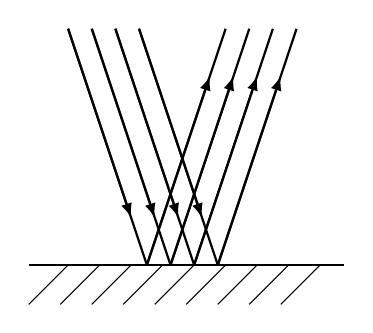
\begin{tikzpicture}
            \draw[thick] (-3, 0) -- (1, 0); % Ground line
            \foreach \i in {-3, -2.6, ..., 0.5} {
                    \draw[] (\i, -0.5) -- (\i+0.5, 0); % Vertical lines
                }
            \foreach \i in {-2.5, -2.2, -1.9, -1.6} {
                    \draw[thick, -latex] (\i, 3) -- (\i +0.8, 0.6);
                    \draw[thick] (\i, 3) -- (\i+1, 0);
                }
            \foreach \i in {-2.5, -2.2, -1.9, -1.6} {
                    \draw[thick, -latex] (\i+1, 0) -- (\i+1.8, 2.4);
                    \draw[thick] (\i+1, 0) -- (\i+2, 3);
                }
        \end{tikzpicture}
        \caption{}
        \label{fig_chp1_reflection_1}
    \end{subfigure}
    \begin{subfigure}{.4\textwidth}
        \centering
        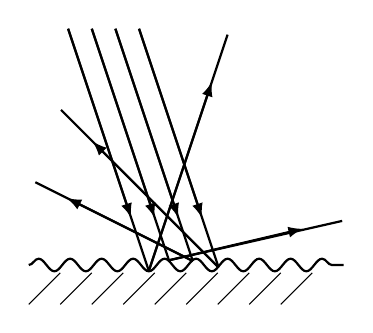
\begin{tikzpicture}
            \draw[thick,decorate,decoration={snake,amplitude=0.8mm,segment length=4mm}] (-3, 0) -- (1, 0); % Ground line
            \foreach \i in {-3, -2.6, ..., 0.5} {
                    \draw[] (\i, -0.5) -- (\i+0.4, -0.1); % Vertical lines
                }

            \foreach \i in {-2.5, -2.2, -1.9, -1.6} {
                    \draw[thick, -latex] (\i, 3) -- (\i +0.8, 0.6);
                }
            \draw[thick] (-2.5, 3) -- (-2.5+1+0.025, 0-0.075);
            \draw[thick, -latex] (-2.5+1+0.025, 0-0.075) -- (-2.5+1+0.025+0.8, 0-0.075+2.4);
            \draw[thick] (-2.5+1+0.025, 0-0.075) -- (-2.5+1+0.025+1, 0-0.075+3);

            \draw[thick] (-2.2, 3) -- (-2.2+1-0.02, 0+0.06);
            \draw[thick] (-2.2+1-0.02, 0+0.06) -- (-2.5+1-0.02+2.5, 0+0.06+0.5);
            \draw[thick, -latex] (-2.2+1-0.02, 0+0.06) -- (-2.5+1-0.02+2, 0+0.06+0.4);

            \draw[thick] (-1.9, 3) -- (-1.9+1-0.017, 0+0.051);
            \draw[thick] (-1.9+1-0.017, 0+0.051) -- (-1.9+1-0.017-2, 0+0.051+1);
            \draw[thick, -latex] (-1.9+1-0.017, 0+0.051) -- (-1.9+1-0.017-1.6, 0+0.051+0.8);

            \draw[thick] (-1.6, 3) -- (-1.6+1+0.01, 0-0.03);
            \draw[thick] (-1.6+1+0.01, 0-0.03) -- (-1.6+1+0.01-2, 0-0.03+2);
            \draw[thick, -latex] (-1.6+1+0.01, 0-0.03) -- (-1.6+1+0.01-1.6, 0-0.03+1.6);
        \end{tikzpicture}
        \caption{}
        \label{fig_chp1_reflection_2}
    \end{subfigure}
    \caption{电磁波的反射示意图 (a) 镜面反射 (b) 漫反射}
    \label{fig_chp1_reflection}
\end{figure}

不同类型的雷达系统会根据目标的散射特性和任务需求选择合适的工作频率,例如:气象雷达通常采用较低频率的 C 波段或 X 波段,以增强对云层和降水等大尺度目标的探测能力;而军事雷达则常使用更高频率的工作体制,以获得更高的空间分辨率和探测精度。

此外,为了降低隐身飞机被雷达探测的概率,通常会采用特殊的设计和材料来减少雷达波的反射。根据电磁波的反射特性,目前主流的隐身技术主要包括以下两种:
\begin{enumerate}
    \item \textbf{外形优化设计}:通过机身外形的精细设计,采用倾斜表面和尖锐棱角结构,尽可能避免出现直角和垂直面,以显著降低雷达波的直接反射。
    \item \textbf{结构与涂层设计}:飞机在一些特定部位(如进气道、雷达罩内部)采用蜂窝状或多孔结构,以增强对雷达波的吸收;同时在机体表面涂覆特殊材料(如吸波材料或漫反射涂层),进一步降低雷达波的反射强度。
\end{enumerate}

利用镜面反射,还可以设计一种特殊的器械,叫作角反射器又名雷达反射器,简称角反。角反可以将入射的电磁波反射回原方向,通常由三个互相垂直的平面组成,如\cref{fig_chp1_corner_reflector}所示。

\begin{figure}[htb!]
    \centering
    \begin{subfigure}{.3\textwidth}
        \centering
        \includegraphics[width=.8\textwidth]{./img/intro/corner_reflector_1.tikz}
        \caption{}
        \label{fig_chp1_corner_reflector_1}
    \end{subfigure}
    \begin{subfigure}{.3\textwidth}
        \centering
        \includegraphics[width=.9\textwidth]{./img/intro/corner_reflector_2.tikz}
        \caption{}
        \label{fig_chp1_corner_reflector_2}
    \end{subfigure}
    \caption{角反射器示意图 (a) 结构示意 (b) 工作原理}
    \label{fig_chp1_corner_reflector}
\end{figure}

事实上,角反在生活中非常常见。比如自行车的尾灯上通常会有一个小的角反射器(如\cref{fig_chp1_bike}所示),用于提高夜间行车的安全性。仔细观察可以发现,这种角反是由大量的小型角反组成的。

\begin{figure}[htb!]
    \centering
    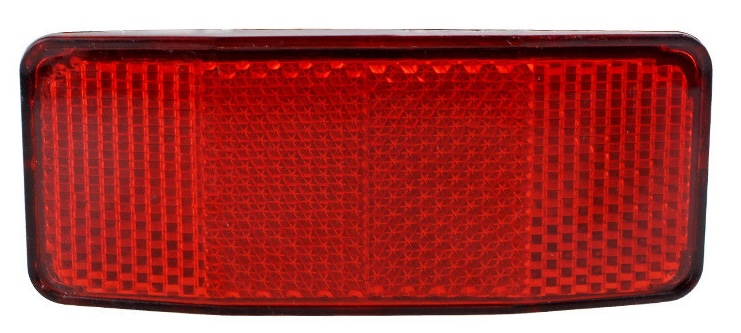
\includegraphics[width=.4\textwidth]{./img/intro/bike.jpeg}
    \caption{自行车尾部的角反射器}
    \label{fig_chp1_bike}
\end{figure}

由于角反可以有效地将入射的电磁波反射回原方向,因此可以提供稳定、明确的强回波信号,通常被用作雷达系统的校准目标,检验雷达设备的测距精度、方向精度和灵敏度。在航海与航空领域,角反射器常用于标识特定位置,如航道、海岸线或机场跑道周围,为雷达导航提供明确的位置标识,提高导航的准确性与安全性。

\subsection{电磁波的折射}

电磁波在不同介质中传播时,由于介质电磁特性的差异,其传播方向会在穿过介质界面时发生改变,这种现象称为折射。折射角的大小取决于入射角和两种介质的折射率。折射率是表征介质对电磁波传播影响的重要参数,定义为电磁波在真空中的传播速度与其在该介质中的传播速度之比,即
\begin{equation}
    n = \frac{c}{v}.
    \label{eq:refraction_index}
\end{equation}

折射是一种常见现象,可以用\textbf{斯涅尔定律}(Snell's Law)来描述。斯涅尔定律表明,当电磁波从一种介质进入另一种介质时,入射角 $\theta_1$、折射角 $\theta_2$ 和两种介质的折射率 $n_1$、$n_2$ 之间满足以下关系:
\begin{equation}
    n_1 \sin \theta_1 = n_2 \sin \theta_2.
    \label{eq:snell_law}
\end{equation}

当电磁波以一个较大的入射角,从折射率较大的介质进入折射率较小的介质时,可能会出现\( n_1 \sin \theta_1 > n_2 \)的情况。此时,即便是\( \theta_2 \) 达到 90°,也无法满足\cref{eq:snell_law},从而导致电磁波无法进入到低折射率介质中,而是全部反射回来。这种现象被称为全反射(Total Internal Reflection)。全反射的条件是入射角大于临界角 $\theta_c$,临界角可以通过以下公式计算:
\begin{equation}
    \sin \theta_c = \frac{n_2}{n_1}.
    \label{eq:critical_angle}
\end{equation}

光纤通信就是利用全反射原理实现的。光纤的核心部分具有较高的折射率,而包裹在外面的包层则具有较低的折射率。当光线以适当的入射角进入光纤时,会发生全反射,从而使光信号在光纤中传播的过程中几乎不损失能量。

在雷达系统中,折射现象也会影响电磁波的传播路径。在海面附近,由于水汽蒸发,会导致近海面小范围内大气湿度随高度锐减,从而形成一个较强的折射率梯度。或是在地面附近,出现逆温层,此时在一个较小的高度范围内,温度随高度增加而迅速升高,同样也会形成一个较强的折射率梯度。

\begin{figure}[htb!]
    \centering
    \includegraphics[width=.7\textwidth]{./img/intro/atmosphere_duct.tikz}
    \caption{大气波导示意图(折射率随海拔升高迅速下降)}
    \label{fig_chp1_atmosphere_duct}
\end{figure}

如\cref{fig_chp1_atmosphere_duct}所示,在折射率梯度的影响下,电磁波的传播路径首先会发生弯曲,导向海面或地面。此后,电磁波被反射,其路径再次弯曲且入射角持续增大,最终因全反射现象而再次返回海面或地面。重复这一过程,电磁波便可以在大气层中沿着地面或海面传播很远的距离,衰减相对而言大大减小。这种现象被称为大气波导(Atmospheric Ducting),也称为大气波导效应。除此以外,大气波导也可能发生在海拔数十米或数百米的空中,基本原理与上述类似,不再赘述。需要注意的是,\cref{fig_chp1_atmosphere_duct}仅为示意图,其中大气的折射率变化并不连续,仅为简化说明而作的分段近似。

当出现大气波导现象时,雷达可以探测到地平线以下的目标。尽管能够探测到目标,但却很难精确地测量目标的距离。如\cref{fig_chp1_radar_ducting}所示,由于大气波导效应,电磁波会沿着地表或海面传播,形成一个弯曲的路径,从而能够探测到地平线以下的目标。
\begin{figure}[htb!]
    \centering
    \includegraphics[width=.6\textwidth]{./img/intro/radar_atmosphere.tikz}
    \caption{雷达超视距探测示意图}
    \label{fig_chp1_radar_ducting}
\end{figure}

\subsection{自由空间路径损耗与大气衰减}

自由空间衰减(Free-Space Path Loss)是指电磁波在自由空间中传播时,由于距离的增加而导致的功率损耗,通常被定义为发射功率与接收功率之间的比值。设有一个发射功率为 $P_t$ 的天线,以球面波形式向外辐射电磁波,则在距离 $r$ 处该电磁波的功率密度 $S$ 可以表示为:
\begin{equation*}
    S = \frac{P_t}{4 \pi r^2}.
    \label{eq:free_space_power_density}
\end{equation*}
而在此处的接收天线接收到的功率 $P_r$ 则与天线的有效面积 $A_e$ 有关,通常可以表示为:
\begin{equation}
    P_r = S A_e = \frac{P_t A_e}{4 \pi r^2},
    \label{eq:free_space_received_power}
\end{equation}
其中,$A_e$ 是接收天线的有效面积。对于一个增益为\( G \)的天线,其有效面积可以表示为:
\begin{equation}
    A_e = \frac{G \lambda^2}{4 \pi},
    \label{eq:effective_area}
\end{equation}
其中 $\lambda$ 是电磁波的波长。考虑一个理想各向同性天线,其增益为 1(即$G=1$),将\cref{eq:effective_area}代入\cref{eq:free_space_received_power},可以得到发射功率和接收功率之间的关系,两者之比即为自由空间路径损耗:
\begin{equation}
    L = \frac{P_t}{P_r} = \left( \frac{4 \pi r}{\lambda} \right)^2 = \left( \frac{4 \pi f r}{c} \right)^2.
    \label{eq:free_space_received_power_final}
\end{equation}

从\cref{eq:free_space_received_power_final}可以看出,自由空间路径损耗与频率 $f$ 的平方成正比。所以想要进行远距离的探测,通常需要使用低频段的电磁波。但低频段的电磁波分辨率较低,无法提供足够的细节信息。因此,在自动驾驶、无人机等应用中,通常会使用高频的毫米波雷达(如24GHz或77GHz),以获得更高的分辨率和精度。相应地,这些雷达的探测距离通常较短,一般在几百米以内。

除此以外,电磁波在大气中传播时还会受到大气衰减的影响。大气衰减是指电磁波在大气中传播时,由于大气中的水汽、氧气、二氧化碳等分子对电磁波的吸收和散射\footnote{散射是指当波遇到空间中物体或介质的不均匀性(如界面、粗糙表面、微粒)时,入射波被扰动,产生新的传播方向和能量分布,从而向多方向重新辐射或传播的物理过程。在广义的波动物理概念中,散射包含了反射和折射引发的辐射场。}作用,导致信号强度的衰减。需要注意的是,大气衰减是指相对于自由空间路径损耗的大气导致的额外功率损耗。大气衰减与频率有关,通常在高频段(如微波和毫米波)更为显著。如\cref{fig_chp1_gaspl}所示,随着频率的增加,大气衰减会显著增加,并且湿空气的衰减比干燥空气更为明显。

\begin{figure}[htb!]
    \centering
    \includegraphics[width=.5\textwidth]{./img/intro/gaspl.tikz}
    \caption{大气衰减曲线\supercite{itu_r_p676_11}(距离1千米,温度$15^\circ$C,气压 $1013$ hPa)}
    \label{fig_chp1_gaspl}
\end{figure}

严格来说,大气本身只能对电磁波产生吸收或散射作用,能量并不会凭空增加。然而,从\cref{fig_chp1_gaspl}可以观察到,衰减数值在某些情况下可能为负值。也就是说,相对于在自由空间中传播,此时电磁波在大气中传播反而损耗更小。这主要是因为,在大气(尤其是近地层)中,温度、湿度等因素引起的折射率梯度会导致电磁波沿地表被导引传播,类似于波导效应,使得能量分布更加集中。因此,即便在较远的距离处,也能够接收到较强的信号。

\subsection{色散现象与多径效应}
电磁波在大气中传播除了会产生传输损耗(衰减)之外,还可能会产生失真。一般来说,产生失真的原因有两个:介质的色散现象和随机多径传输导致的干涉效应。

对于同一个介质,不同频率的电磁波在该介质中的传播速度有可能是不同的。这就会导致在传播的过程中,雷达发射的信号波形产生畸变,这种现象称为色散现象(Dispersion)。色散现象的一个典型例子是光在玻璃中的传播:当白光通过棱镜时,不同波长的光会以不同的速度传播,从而导致光线分散成彩虹色谱。如果我们将传播介质看作是一个线性系统,那么该系统的频率响应是非线性相位的。而对于一个非线性相位的系统,其输出信号的波形相较于输入信号波形会发生畸变。
\begin{figure}[htb!]
    \centering
    \begin{subfigure}{.3\textwidth}
        \centering
        \includegraphics[width=.9\textwidth]{./img/intro/filter1.tikz}
        \includegraphics[width=.9\textwidth]{./img/intro/filter4.tikz}
        \caption{}
        \label{fig_chp1_filter_1}
    \end{subfigure}
    \begin{subfigure}{.3\textwidth}
        \centering
        \includegraphics[width=.9\textwidth]{./img/intro/filter2.tikz}
        \includegraphics[width=.9\textwidth]{./img/intro/filter4.tikz}
        \caption{}
        \label{fig_chp1_filter_2}
    \end{subfigure}
    \begin{subfigure}{.3\textwidth}
        \centering
        \includegraphics[width=.9\textwidth]{./img/intro/filter3.tikz}
        \includegraphics[width=.9\textwidth]{./img/intro/filter4.tikz}
        \caption{}
        \label{fig_chp1_filter_3}
    \end{subfigure}
    \caption{色散现象示意图 (a) 原始信号及频谱 (b) 无色散滤波器输出 (c) 有色散滤波器输出}
    \label{fig_chp1_filter}
\end{figure}

如\cref{fig_chp1_filter}所示,可以看到,对于一个全通滤波器,如果相位响应是线性的,那么输出信号的波形与输入信号的波形相同,仅存在时延;反之,如果滤波器的相位响应是非线性的,那么输出信号的波形会发生畸变,但频谱仍然保持不变。不过大气对常见的雷达工作频率的色散效应并不明显,通常可以忽略不计。比如最靠近地表的对流层,其对20GHz以下的电磁波基本上是无色散的。

% TODO: 多径效应可以展开讲一讲,给一个例子
此外,多径效应(Multipath Effect),则是指电磁波在传播过程中,由于遇到障碍物或地形的反射、折射和散射等作用,导致同一信号在不同路径上到达接收天线的现象,如\cref{fig_chp1_multipath}所示。多径效应会导致接收信号的相位和幅度发生变化,从而引起信号的干扰和失真。严重时,不同路径上的信号可能会相互抵消,导致接收信号的强度显著降低。

\begin{figure}[htb!]
    \centering
    \includegraphics[width=.5\textwidth]{./img/intro/multipath.tikz}
    \caption{多径效应示意图}
    \label{fig_chp1_multipath}
\end{figure}

\section{雷达方程}
雷达方程(Radar Equation)是雷达系统最核心的工程公式之一,用于定量描述雷达发射、传播、反射和接收信号之间的功率关系。它既揭示了影响探测距离和信号强度的主要物理量,也为雷达系统设计提供了基础依据。本节以最简单的单站雷达(即发射、接收天线距离很近,甚至共用同一个天线)为例,详细介绍雷达方程的推导过程。


\begin{figure}[htb!]
    \centering
    \begin{subfigure}{.7\textwidth}
        \centering
        \begin{tikzpicture}
            \begin{axis}[
                    xlabel=$ x $, ylabel=$ y $,
                    ticklabel style={font=\small},
                    label style={font=\small},
                    axis equal image,
                    axis lines=none,
                    legend cell align=left,
                    legend style={
                            anchor=north east,
                            font=\tiny,
                            draw=none,
                            fill=none
                        }
                ]
                \addplot graphics [xmin=-0.5, xmax=0.5, ymin=-0.5, ymax=0.5] {img/radar.png};
                \addplot graphics [xmin=2.5, xmax=3.5, ymin=0.5, ymax=1.5] {img/target.png};
                % light from radar to target and back
                \addplot[thick, -latex, c1] coordinates {(0.5, 0.3) (2.5, 0.9)} node[midway, above=3pt, black] {距离为\( r \)};
                % \addplot[thick, -latex, c2] coordinates {(2.5, 0.8) (0.5, 0.2)} node[midway, below=3pt, black] {\tiny 自由空间损耗\( L \)};
                \node at (axis cs:0, 0.5) [font=\tiny] {发射增益\( G_t \)};
                \node at (axis cs:0, 0.7) [font=\tiny] {发射功率\( P_t \)};
                \node at (axis cs:3, 1.5) [font=\tiny] {功率密度\( S_t = \frac{P_t G_t}{4 \pi r^2} \)};
                \node at (axis cs:3, 0.5) [font=\tiny] {目标雷达截面积\( \sigma \)};
            \end{axis}
        \end{tikzpicture}
        \caption{}
        \label{fig_chp1_radar_equation_1}
    \end{subfigure}
    \begin{subfigure}{.7\textwidth}
        \centering
        \begin{tikzpicture}
            \begin{axis}[
                    xlabel=$ x $, ylabel=$ y $,
                    ticklabel style={font=\small},
                    label style={font=\small},
                    axis equal image,
                    axis lines=none,
                    legend cell align=left,
                    legend style={
                            anchor=north east,
                            font=\tiny,
                            draw=none,
                            fill=none
                        }
                ]
                \addplot graphics [xmin=-0.5, xmax=0.5, ymin=-0.5, ymax=0.5] {img/radar.png};
                \addplot graphics [xmin=2.5, xmax=3.5, ymin=0.5, ymax=1.5] {img/target.png};
                % light from radar to target and back
                \addplot[thick, -latex, c2] coordinates {(2.5, 0.8) (0.5, 0.2)} node[midway, below=3pt, black] {距离为\( r \)};
                \node at (axis cs:0, -0.5) [font=\tiny] {接收增益\( G_r \)};
                \node at (axis cs:3, 1.5) [font=\tiny] {反射功率\( P_s = S_t \sigma \)};
                \node at (axis cs:3, 0.5) [font=\tiny] {目标雷达截面积\( \sigma \)};
                \node at (axis cs:0, 0.5) [font=\tiny] {功率密度\( S_r = \frac{P_s}{4 \pi r^2} \)};
                \node at (axis cs:0, 0.7) [font=\tiny] {接收功率\( P_r = S_r A_e \)};
            \end{axis}
        \end{tikzpicture}
        \caption{}
        \label{fig_chp1_radar_equation_2}
    \end{subfigure}
    \caption{雷达方程示意图 (a) 雷达发射与目标反射 (b) 目标反射与雷达接收}
    \label{fig_chp1_radar_equation}
\end{figure}

如\cref{fig_chp1_radar_equation_1}所示,设雷达系统的发射功率为 $P_t$,且发射天线增益为 $G_t$,那么在距离雷达发射天线 $r$ 处的功率密度 $S_t$ 可以表示为:
\begin{equation*}
    S_t = \frac{P_t G_t}{4 \pi r^2}.
    \label{eq:radar_power_density}
\end{equation*}
而在此处的目标会将雷达发射的电磁波,以镜面反射、漫反射、体散射等方式返回给雷达接收天线,方便起见这里统称散射。由于目标的结构和材料千差万别,很难直接计算目标的散射特性,但可以使用雷达截面积(Radar Cross-Section, RCS)来整体性地描述目标对雷达波的散射能力。简而言之,如果目标的雷达截面积为 $\sigma$,那么目标散射的电磁波的总功率 $P_s$ 可以表示为:
\begin{equation*}
    P_s = S_t \sigma.
    \label{eq:radar_received_power}
\end{equation*}

因此,如\cref{fig_chp1_radar_equation_2}所示,在接收天线处目标散射回来的电磁波的功率密度 $S_r$ 可以表示为:
\begin{equation*}
    S_r = \frac{P_s}{4 \pi r^2} = \frac{P_t G_t \sigma}{(4 \pi r^2)^2}.
    \label{eq:radar_received_power_density}
\end{equation*}
若接收天线的增益为 $G_r$,根据天线增益和有效面积的关系,接收天线的有效面积 $A_e$ 可以表示为:
\begin{equation}
    A_e = \frac{G_r \lambda^2}{4 \pi}.
    \label{eq:radar_effective_area}
\end{equation}
将接收天线有效面积\( A_e \)与目标散射回来的电磁波的功率密度\( S_r \)相乘,便可以得到接收天线接收到的功率 $P_r$ 为:
\begin{equation}
    P_r = A_e S_r  = \frac{G_r \lambda^2}{4 \pi} \cdot \frac{P_t G_t \sigma}{(4 \pi r^2)^2}.
    \label{eq:radar_received_power_final}
\end{equation}
将\cref{eq:radar_received_power_final}整理后,可以得到雷达方程的标准形式:
\begin{equation}
    P_r = \frac{P_t G_t G_r \lambda^2 \sigma}{(4 \pi)^3 r^4}.
    \label{eq:radar_equation}
\end{equation}

假设雷达能够检测的最小接收功率为 $P_{\text{min}}$,则根据\cref{eq:radar_equation},可以得到雷达的最大探测距离 $r_{\text{max}}$ 为:
\begin{equation}
    r_{\text{max}} = \left( \frac{P_t G_t G_r \lambda^2 \sigma}{(4 \pi)^3 P_{\text{min}}} \right)^{1/4}.
    \label{eq:radar_max_range}
\end{equation}
从\cref{eq:radar_max_range}可以看出,雷达的最大探测距离与发射功率 $P_t$、发射天线增益 $G_t$、接收天线增益 $G_r$、发射信号波长 $\lambda$ 以及目标的雷达截面积 $\sigma$ 成正相关,而与接收机的最小接收功率 $P_{\text{min}}$ 成负相关。

雷达方程与自由空间损耗有着密切的联系:显然,电磁波经历了从雷达到目标再从目标到雷达这两步传播过程,其中经历了两次自由空间损耗。如果我们将目标也看作是一个天线,那么目标的雷达截面积 $\sigma$ 则对应了天线的有效面积。因此,根据\cref{eq:radar_effective_area},我们可以得到目标作为一个天线时的增益为
\[
    G_s =  \frac{4 \pi \sigma}{\lambda^2}.
\]
此时,我们可以将发射功率与接收功率的比值写为
\begin{equation}
    \frac{P_t}{P_r} = \frac{(4 \pi)^3 r^4}{G_t G_r \lambda^2 \sigma} =\frac{(4 \pi r)^4}{\lambda^4 G_t G_r G_s} = \frac{L^2}{G_t G_r G_s},
    \label{eq:radar_equation_gain}
\end{equation}
其中 $L$ 是自由空间路径损耗,表达式见\cref{eq:free_space_received_power_final}。

\begin{figure}[htb!]
    \centering
    % \includegraphics[width=.4\textwidth]{./img}
    \begin{tikzpicture}
        \begin{axis}[
                xlabel=$ x $, ylabel=$ y $,
                ticklabel style={font=\small},
                label style={font=\small},
                axis equal image,
                axis lines=none,
                legend cell align=left,
                legend style={
                        anchor=north east,
                        font=\tiny,
                        draw=none,
                        fill=none
                    }
            ]
            \addplot graphics [xmin=-0.5, xmax=0.5, ymin=-0.5, ymax=0.5] {img/radar.png};
            \addplot graphics [xmin=2.5, xmax=3.5, ymin=0.5, ymax=1.5] {img/target.png};
            % light from radar to target and back
            \addplot[thick, -latex, c1] coordinates {(0.5, 0.3) (2.5, 0.9)} node[midway, above=3pt, black] {\tiny 自由空间损耗\( L \)};
            \addplot[thick, -latex, c2] coordinates {(2.5, 0.8) (0.5, 0.2)} node[midway, below=3pt, black] {\tiny 自由空间损耗\( L \)};
            \node at (axis cs:0, 0.5) [font=\tiny] {发射增益\( G_t \)};
            \node at (axis cs:0, -0.5) [font=\tiny] {接收增益\( G_r \)};
            \node at (axis cs:3, 0.5) [font=\tiny] {目标增益\( G_s \)};
        \end{axis}
    \end{tikzpicture}
    \caption{雷达方程与自由空间损耗}
    \label{fig_chp1_radar_equation_gain}
\end{figure}

如\cref{fig_chp1_radar_equation_gain}所示,\cref{eq:radar_equation_gain}具有明确的物理意义:在雷达系统中,发射机首先向外辐射电磁波,信号在传播至目标的过程中经历了一次功率损耗,记为 $L$;目标对入射电磁波产生散射,回波信号返回接收天线时,又沿相同路径传播一次,再次损耗 $L$ 倍。若仅考虑自由空间传播损耗,总的路径损耗应为 $L^2$。然而,实际系统中发射天线和接收天线均具有方向性增益,目标本身的散射特性也不等价于理想的各向同性天线,因此这些因素会对功率分布产生修正。综合考虑这些增益因素后,功率项应再除以 $G_t G_r G_s$,从而得到更为准确的雷达方程。

\section{小结}

本章主要介绍了雷达及其相关的基本概念、组成原理与工作特性。首先,回顾了雷达的起源,阐述了雷达利用电磁波反射实现目标探测的基本思想,并简要介绍了赫兹实验证实电磁波存在的过程。随后,系统地讲解了现代雷达的基本组成及其工作流程,包括波形产生、发射、接收及信号处理等环节,重点分析了不同工作频率雷达的应用特点。在此基础上,进一步探讨了电磁波在传播过程中的几种典型物理现象:反射、折射、大气波导、色散以及多径效应,并说明了这些现象对雷达探测的影响。最后,推导了雷达方程,揭示了雷达系统中各个参数之间的关系,为后续章节的深入学习奠定了基础。通过本章的学习,读者应能初步理解雷达的工作原理及其在实际应用中的重要性,为后续章节的深入研究做好准备。